% !TEX encoding = UTF-8 Unicode
% !TEX root = ../../relatorio.tex

%% Responsavel:

\subsection{Questão 3.21}

How does your system compare to ours? What run-times does your system get for matrix-vector multiplication? What kind of variability do you see in the times for a given value of \texttt{comm\_sz} and $n$? Do the results tend to cluster around the minimum, the mean, or the median?

\begin{table}[h!]
\centering
\begin{tabular}{|l|lllll|}
    \hline
     & \multicolumn{5}{c|}{Ordem da Matriz}\\
     \hline
    comm\_sz & 1024 & 2048 & 4096 & 8192 & 16384 \\
    \hline
    1 & 3.7561 & 12.8853 & 52.0139 & 210.4686 & 846.9655 \\
    2 & 2.0700 & 10.2071 & 41.1858 & 107.3081 & 438.0811 \\
    4 & 1.7275 & 6.8219 & 25.0998 & 64.2229 & 245.5204 \\
    8 & 1.7007 & 4.1896 & 14.3932 & 56.5015 & 219.8544 \\
    16 & 2.1960 & 6.0016 & 20.8711 & 76.8699 & 236.1451 \\
    \hline
\end{tabular}
\caption{Tempo de execução}
\label{tab:timeq21}
\end{table}

A medida que o comm\_sz aumenta, é possível ver que o tempo de execução diminui. Contudo, a execução nem sempre tem um comportamento constante. Isso pode ser observado na Figura \ref{fig:comp}.

\begin{figure}[h!]
\centering
\begin{subfigure}{.5\textwidth}
  \centering
  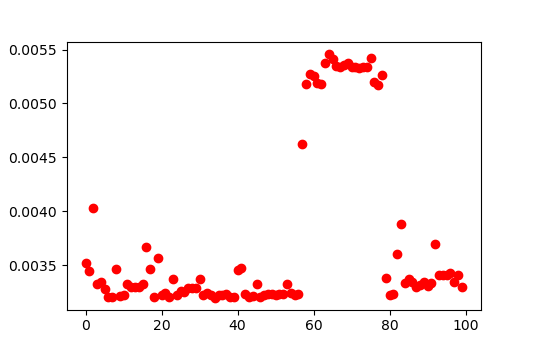
\includegraphics[width=.9\linewidth]{sections/q3.21/imgs/fig1-1024.png}
  \caption{\texttt{comm\_sz} = 1, Ordem = 1024, (s)}
  \label{fig:sub1}
\end{subfigure}%
\begin{subfigure}{.5\textwidth}
  \centering
  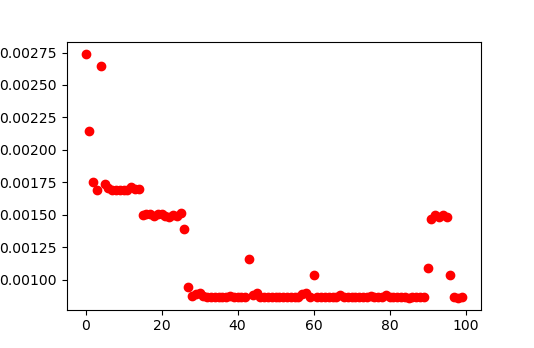
\includegraphics[width=.9\linewidth]{sections/q3.21/imgs/fig4-1024.png}
  \caption{\texttt{comm\_sz} = 4, Ordem = 1024, (s)}
  \label{fig:sub2}
\end{subfigure}
\begin{subfigure}{.5\textwidth}
  \centering
  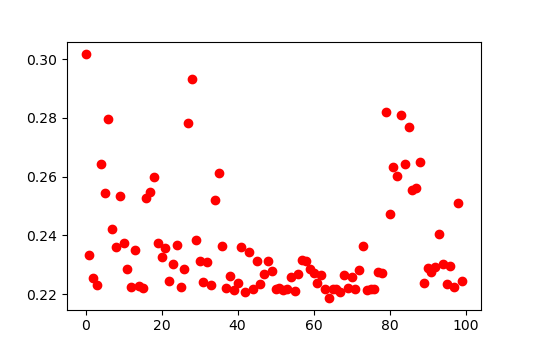
\includegraphics[width=.9\linewidth]{sections/q3.21/imgs/fig16-16384.png}
  \caption{\texttt{comm\_sz} = 16, Ordem = 16384, (s)}
  \label{fig:sub3}
\end{subfigure}
\caption{Comportamento dos tempos de execução}
\label{fig:comp}
\end{figure}


%%% Local Variables:
%%% mode: latex
%%% TeX-master: "../../relatorio"
%%% End:
